\documentclass[conference]{IEEEtran}

\usepackage{glossaries}
\usepackage[usenames,dvipsnames,svgnames,table]{xcolor}
\usepackage[pdftex,draft]{hyperref}
\usepackage[pdftex]{graphicx}
\usepackage{algpseudocode}
% \usepackage{enumitem}
% System names
\newglossaryentry{name}
{%
    name=tutoron,
    description={skill-specific text augmentation to existing tutorials that enable just-in-time training for a supplemental skill a tutorial glosses over.}
}
\newglossaryentry{exp}
{%
    name=micro-explanation,
    description={explanation or demonstration generated to help a programmer better understand an explainable region of code.}
}

\newcommand\condcap[1]{\ifnum\ifhmode\spacefactor\else2000\fi>1000 \uppercase{#1}\else#1\fi}
\newcommand{\systemname}{\Glspl{name}}
\newcommand{\user}{Colin}
\newcommand{\userpro}{\condcap{h}e}
\newcommand{\userpos}{\condcap{h}is}
\newcommand{\urltarget}{site.com}
\newcommand{\headrow}[1]{\scriptsize\textbf{#1}}
\newcommand{\qs}{\textquotesingle}

% Formatting tables
\newcommand*{\thead}[1]{\multicolumn{1}{|c|}{\bfseries #1}}
\def\arraystretch{1.5}
\setlength\tabcolsep{4pt}

% Formatting code
\newcommand{\snippet}[1]{%
\vspace{.3em}
\framebox[\linewidth]{%
    \begin{minipage}{.95\linewidth}
        \begin{hangparas}{.25in}{1}
        \small\texttt{#1}
        \end{hangparas}
    \end{minipage}
}
}

% Revision Macros
\newcommand{\andrew}[1]{{\color{red}\textbf{AH\@: #1}\normalfont}}
% \newcommand{\andrew}[1]{{\color{red}\textbf{}\normalfont}}
\newcommand{\bjoern}[1]{{\color{blue}\textbf{BH\@: #1}\normalfont}}
\newcommand{\marti}[1]{{\color{brown}\textbf{MH\@: #1}\normalfont}}
\newcommand{\appachu}[1]{{\color{purple}\textbf{CA\@: #1}\normalfont}}
\newcommand{\shortchange}[1]{{\color{OliveGreen}\textbf{#1}\normalfont}}
% \newcommand{\shortchange}[1]{{#1}}
\newenvironment{changes}{\shortchange\bgroup}{\egroup}

\makeglossaries

\ifCLASSOPTIONcompsoc
  \usepackage[tight,normalsize,sf,SF]{subfigure}
\else
  \usepackage[tight,footnotesize]{subfigure}
\fi

% correct bad hyphenation here
\hyphenation{op-tical net-works semi-conduc-tor}

\begin{document}
\title{\Glspl{name}: Automatic Augmentation and Clarifications for Programming Tutorials}

% author names and affiliations
% use a multiple column layout for up to three different
% affiliations
\author{
\IEEEauthorblockN{Author 1}
\IEEEauthorblockA{Division \\
School \\
City, ST ZIP\\
Email: person@url.org}
\and
\IEEEauthorblockN{Author 2}
\IEEEauthorblockA{Division \\
School \\
City, ST ZIP\\
Email: person@url.org}
}

% make the title area
\maketitle

\begin{abstract}

Programmers frequently turn to tutorials to learn frameworks and find new approaches to solving problems.
However, today's ``wild'' blog-based tutorials can contain pitfalls, errors, and underexplained concepts that require programmers to spend time looking up external documentation and debugging errors others have already encountered.
While the value of community cultivation and maintenance of knowledge bases and annotations on the web is well-explored, we suggest that \emph{code-centered markup} of the web enables new ways of detecting pitfalls, generating custom help, and sharing information.
In this paper, we describe \Glspl{name} framework, a system for community-led augmentation and maintenance of programming tutorial documentation.
By implementing a variety of \Gls{name} generators, we outline a design space of tools for code-based online tutorial augmentations, from Simple \Glspl{name} for trivial in-browser code annotation, to Power \Glspl{name} for automatically generating explanations of code fragments found anywhere on the web.
Through an in-lab qualitative study, we demonstrate that community-sourced \Glspl{name} can be fast to create and enable significant time savings for tutorial readers.
With a quantitative analysis of Power \Glspl{name}, we show that automatic augmentations can reach across dozens of tutorials for key programming tasks.
\andrew{Careful as to whether we define \Glspl{name} as a framework, as individual augmentations, or something else.
Be consistent!}

\end{abstract}


% For peerreview papers, this IEEEtran command inserts a page break and
% creates the second title. It will be ignored for other modes.
\IEEEpeerreviewmaketitle

\section{Introduction}

\andrew{We can include a mention that we replicate the spirit of modern-day templating engines when providing the ability to generate descriptions within the DOM.  Can we work this into the design?}
\andrew{We can also phrase this paper as techniques for automatic augmentation of tutorials.}

The proliferation of programming resources on the web has enabled the growth of an enormous programmer community.
Relevant content for solving programming problems resides across an abundance of tutorials, MOOCS, programming examples, Q\&A sites and technical blogs.
These resources are popular for programmers of varying skill levels and fill in the inadequacies of traditional documentation and formal references.
Today's coding workflow contrasts starkly from that of a decade ago.
Programmers retrieve web resources and engage in self-led learning during each iteration of code implementation and foraging~\cite{brandt_two_2009}~\cite{brandt_example-centric_2010}.

A search for a solution to a programming problem begins with a Google search, leading to blog posts, tutorials, reference documentation, forums, and online Q\&As.
Searchers assess the relevance of online examples prior to extensive manual inspection of documents in multiple ways.
First, they rely on their search engine to rank results such that those at the top of the page will provide a relevant solution.
Second, they examine the textual excerpts returned with each result for additional context.
Third, for online Q\&A like StackOverflow, they assess which examples will be most helpful based on votes and user reputation.

Whether a programmer can successfully understand and integrate code examples into his code depends on many factors.
Code examples should build upon familiar libraries and explanatory text should use known terms or provide a definition of them.
If they contain errors, the programmer should be able to find related examples with the same classes and functions to check his work.
The programmer may already know whether he is looking for long textual responses or short code snippets. 
Modern search engines should offer a way for a user to quickly and effectively assess which examples contain a promising amount of explanation, usable libraries and terminology.

\andrew{TODO: adapt this to our new system description.}
We develop \systemname{}, a search user interface that provides solutions to these problems through visual features.
Our tool represents text and code of code examples in colored columns to allow easy assessment of content distribution for each search result.
It generates charts of commonly used classes and coding concepts to help users with early detection of frequently used dependencies used for solving a problem.
A preview panel provides a way to rapidly skim through the content of multiple examples without requiring navigation through tabs or links.
A snippet bank enables users to maintain an in-tab history of promising code segments and explanations and to compare two examples side-by-side.
\systemname{} leverages the StackExchange API to gain access to answers to over 700,000 questions on StackOverflow, providing an overview of dozens of relevant answers with each query.

\andrew{This needs to change too}
This work concludes with a 4-subject user study to evaluate the usefulness of our tool.
We determine that \systemname{} enables tasks like finding the most commonly used classes across examples where a baseline search interface does not.
Participants find it useful to be able to pinpoint structural code elements like functions, viewing them across many examples at once.
They also see value using the system in the early stages of learning when required to use libraries in unfamiliar programming tasks.
We finish with a discussion of future directions, focusing on the challenges of encouraging users to use a breadth-first approach in when finding programming solutions.

\section{Related Work}

Our work is related to research in multiple directions.
In this paper, we compare our work to past research in the automatic explanation of code and demonstration of code.

\subsection{Automatic Explanation of Code}

Most closely related to our work is Webcrystal~\cite{chang_webcrystal_2012}, a tool that assists web authors with low-level programming tasks required to learn from and reuse examples.  
Webcrystal generates human-readable textual answers to user's ``how'' questions about how to recreate aspects of selected HTML elements as well as customized code snippets for the user's to recreate the design.
Similar to Webcrystal, we generate human-readable representations of code to help programmers learn from and reuse online examples.
In contrast to Webcrystal, we focus on the task of describing several small languages instead of DOMs, focusing on generalizable design patterns for explanations that can apply to generating explanation support for other programming languages in the future.

In its technical approach, our work also relates to recent work on generating natural language explanations of code and software engineering artifacts~\cite{sridhara_automatically_2011,burden_natural_2011,sridhara_towards_2010,kamimura_towards_2013,mcburney_automatic_2014,sridhara_generating_2011,haiduc_supporting_2010,moreno_automatic_2013}.
This body of work focuses on how to reduce the amount of time developers spend reading poorly-documented code by automatically summarizing Java methods~\cite{sridhara_towards_2010}, blocks of code~\cite{sridhara_automatically_2011}, method parameters~\cite{sridhara_generating_2011}, and classes~\cite{moreno_automatic_2013}.
Similar to ourselves, Sridhara et al. consider how to detect explainable code prior to generating descriptions~\cite{sridhara_automatically_2011,sridhara_towards_2010}.
However, their code detection process emphasizes summarization of methods and blocks of code rather than locating instances of a language in a heterogeneous code snippet.
In addition, we distance ourselves from this past work by examining the code explanation problem from the perspective of unexplained code on the web.
This enables us to test out and propose guidelines for detecting, parsing and explaining code by minding the constraints and affordances of the language.

\subsection{Automatic Demonstration of Code}

Software visualization has a long history of producing visual representations of code for varying purposes~\cite{sorva_visual_2012}.
PythonTutor~\cite{guo_online_2013} is one current example of a programming visualization tool for CS education.
Embeddable within a webpage, it supports simultaneous viewing of program source code, program execution, visual representations of Python objects, and program output.
More recently, Ou et al. produced visualizations of arbitrary pointer-based data structures in the heap~\cite{ou_interactive_2015}.
Beyond visualizations, code can be represented by discrete structures.
Dantoni et al.~\cite{dantoni_how_2015} demonstrate how to create counterexamples of system behaviors for helpful feedback for computer science students completing automata design problems.
We draw inspiration broadly from this past work in both visualization and example generation to automatically produce demonstrations of regular expresions and HTML.
We believe we are the first to consider building demonstrations from the perspective of writing design guidelines for micro-explanations of code found in online programming help.
\section{Scenario}

\andrew{Create some graphics here of tutorials before and after tutoroids, \emph{highlighting} the text that is created by tutoroids.}.

Jim is developing a Bluetooth Low Energy app for Android and wants to find a code example that will easily help him write serial data from an Android app to an Arduino.
He visits the \systemname{} example explorer, which has one million Java examples across many topics.
He enters the query \emph{Bluetooth Android write serial}.

Just like on Stack Overflow, question titles are returned with text snippets that highlight his query terms.
For these questions, there are around 10 different answers that he thinks might be applicable to his problem, but he doesn't know where to start.
Each answer is augmented with a \systemname{}, bars that visually show the complexity and content of the examples.
He toggles a button that lets him view all of the \systemname{} side by side without the interspersed title and surrogate text.
Jim knows he wants to find and answer fast, so he starts by sorting the \systemname{} entries based on their length.
He quickly finds the shortest one, and with the scrolling tooltip, he inspects the code snippets at each point to see if it contains the content that will help him solve his problem.

The tooltip shows him that this example is far too short -- it's just a correction to a previous code example.
Jim sees some examples at the bottom that are interesting.
He also recalls that the Android library for Bluetooth code is org.android.bluetoothlowenergy.
He decides that the relevant code examples will contain this library.
So, he enters this library name in a search widget off to the side.
The code examples that use the bluetoothlowenergy library are focused with a light tint.
Furthermore, the locations in the code with the bluetoothlowenergy usage are highlighted.
Jim scrolls his tooltip over these locations to gain an idea of how the library is invoked to solve his problem.

From another view above the \emph{Library Inclusion} view, he adds a library using the \emph{Library Exclusion} view.
By doing this, he makes sure that none of the code examples returned include a deprecated library, com.android.bluetooth.
He removes from the listing 2 of the old examples that include this library.

When inspecting how the code examples invoke Bluetooth by hovering the mouse over the bar for org.android.bluetoothlowenergy, he notices something untoward.
Many of these examples perform the command BluetoothAdapter.read().
However, Jim recognizes that to solve his problem, he will need to access a method called BluetoothAdapter.write(), the complement to read().
He types in the \emph{Highlight Text} box the term \emph{write}.
In each of the \systemname{}, the location of the word is highlighted, just like it would be in a vertical scrollbar on the side of the page.
With this, Jim finds an example that not only leverages the libraries that he needs, but also invokes the commands he expects will be the most helpful.

Jim is left with only a few candidate code examples at this point.
He would love an example that could be plugged right into his code.
He looks at the right column of the search results to see an 'X' marking all of the code examples that cannot compile.
He chooses the one code example that includes the libraries and commands that he wants, and the code.
From this, he has found a transplantable code example that will satisfy his needs, all without having to click through a single search result.
Jim pastes this into his source code editor, compiles, and writes to his Bluetooth Low Energy device with minimal additional effort.
% \section{Preliminary Study}

\andrew{Do the following studies. Numbers included below are optimistic placeholders.}
\andrew{A table would be great to summarize these results.}

StackOverflow is a popular online Q\&A site for programmers to ask and answer progrmaming problems, with more than 16 million answers to more than 9 million questions.

\begin{itemize}
\item Through an inspection of the top 200 most-viewed posts on StackOverflow, we find 10 \emph{micro-languages} that are not included as tags of the post, but that are used incidentally, including command lines, SQL, and regular expressions. \marti{unclear wording; also, do you want to mention wget explicitly here as a pointer forward?}
\item In addition, out of 100 top-rated posts related to Python that include regular expressions, we found that 50\% did not include any description of what the regular expression was doing, and 75\% provided a concise description or less.\marti{do we want a bullet for command lines?}
(We can do the same for CSS in jQuery selections.)
\end{itemize}

For users who find code with unexplained languages and syntax, we propose that we can reduce the cost of looking up supplemental information that explains these micro-languages by automatically generating relevant explanations of this code on the fly.

\section{Parsing StackOverflow Answers}

\systemname{} allows users to perform queries on answers to over 700,000 Java questions indexed on StackOveflow, an online programming Q\&A site.
On StackOverflow, users pose questions to the community.
Other members provide answers, which are voted to be helpful or unhelpful.
One question can have multiple answers.
For \systemname{}, answers to questions related to a user's query make up the code examples they search through for solutions.

Using StackOverflow as a central corpus for code examples offered three advantages.
First, developers can access the the site's full answer index the StackExchange API, which allows 10,000 queries per day with authentication.
Second, in our own experience we have found StackOverflow to provide high quality answers over a range of topics.
Third, each example is \emph{preformatted} into distinct code and text sections when authored in a StackOverflow markdown editor, making separation of text and code in examples simple.
We restrict ourselves to only Java-related answers on StackOverflow, the programming language with the most questions.

We parse three classes of features from examples:

\emph{Content blocks and types}. 
StackOverflow answers have three types of content (Figure~\ref{fig:so_answer}): explanatory text, source code, and in-code comments.
Explanatory text is wrapped in HTML \emph{\textless{}p\textgreater{}} and \emph{\textless{}li\textgreater{}} elements.
It can be divided into sentences by splitting this content on periods.
Code is wrapped in \emph{\textless{}pre\textgreater{}} elements, which can be divided into lines by the newline character.
In-code comments can be detected through regular expression matching of double-slash and slash-star patterns.

\begin{figure}
 \centering
 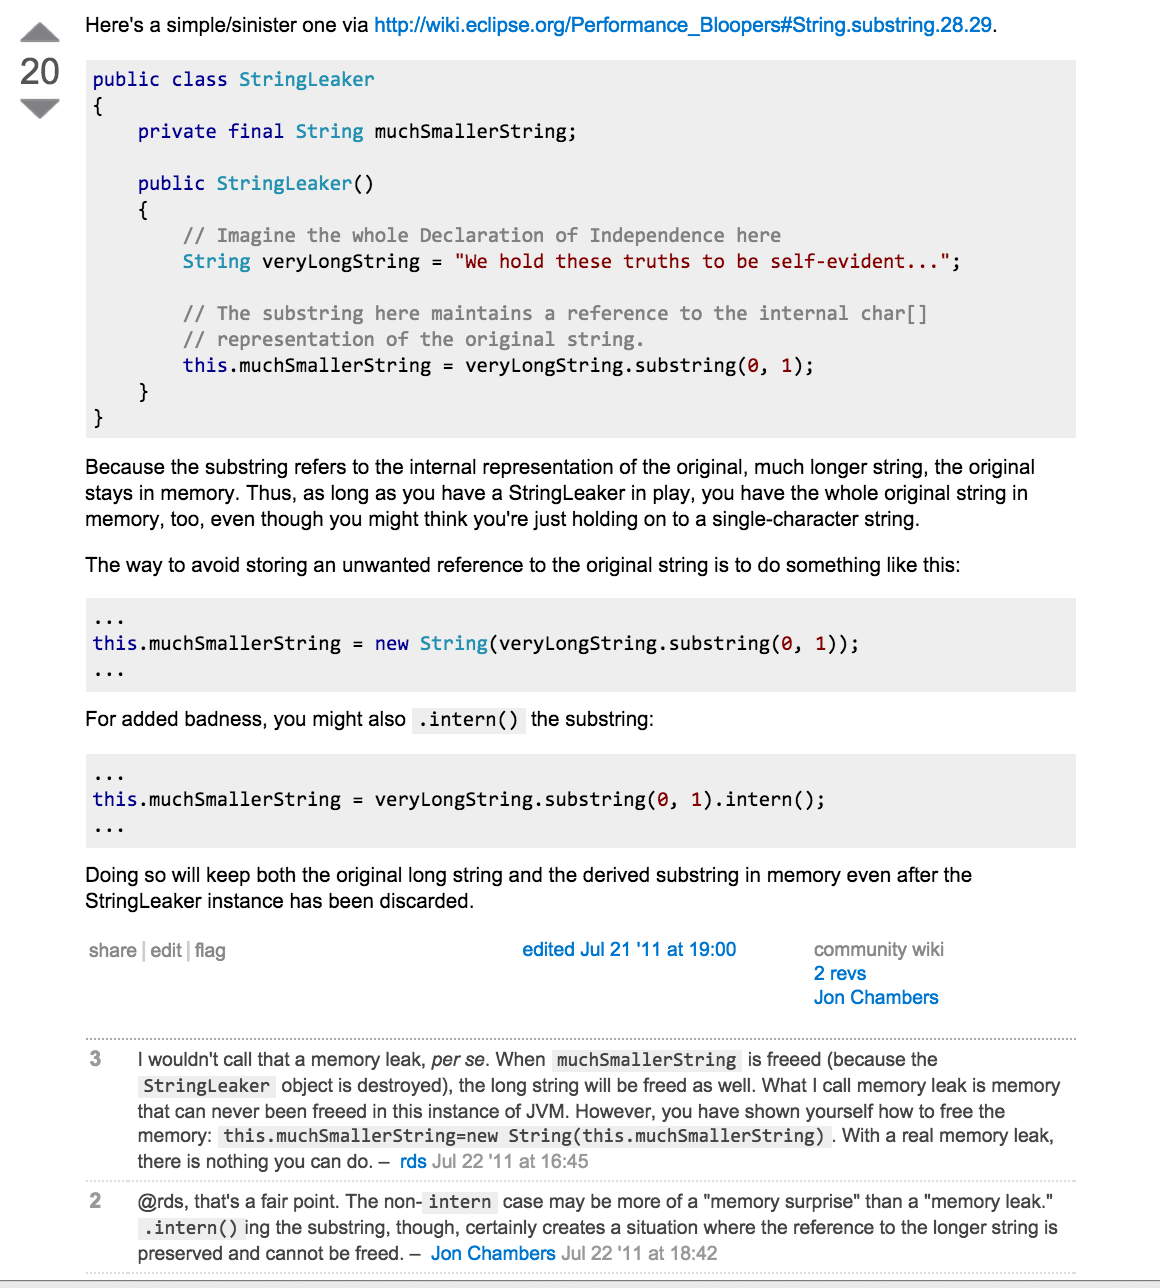
\includegraphics[width=.85\columnwidth]{figures/so_answer}
 \caption{An answer to a Stack Overflow question.  This example contains lines of code, explanatory text, and inline code comments.}
 \label{fig:so_answer}
\end{figure}

\emph{Class usage}.
After extracting content blocks from an answer, we detect classes.
First, we search in the explanatory text for single-word phrases contained within \emph{\textless{}code\textgreater{}} tags.
If the term begins with a capital letter, we assume it to be a Java class.
Second, we perform a regular expression max on the code to detect all class names used in the declaration of a variable, or coupled with a \emph{new} keyword to instantiate an object.

\emph{Concept usage}.
We detect whether examples use concepts learned in the CS1 classroom like loops, functions and objects by using regular expressions for Java keywords, symbols, and sequences of tokens.

We expect that more accurate detection of classes and concepts could be achieved by parsing code examples to their abstract syntax trees and inspecting the nodes of this tree.
However, we note that many code snippets on StackOverflow are incomplete and cannot be compiled.
For this reason, we used regular expression matching to capture class and concept use for this version of \systemname{}.
\section{Authors and Readers in the \Gls{name} Ecosystem}

In the current incarnation of \glspl{name}, an author of code documentation writes a \gls{name} in order to adaptively describe  code programmers find while they browse the web.
A \gls{name} is an engine for generating explanations or demonstrations of code for a specific language, accessible as a simple web API.
When queried with the text of a web page, a \gls{name} detects explainable regions of the language, parses them, and returns explanations for each region as formatted HTML that can be viewed in a tooltip.

\begin{figure}
%%\centering
    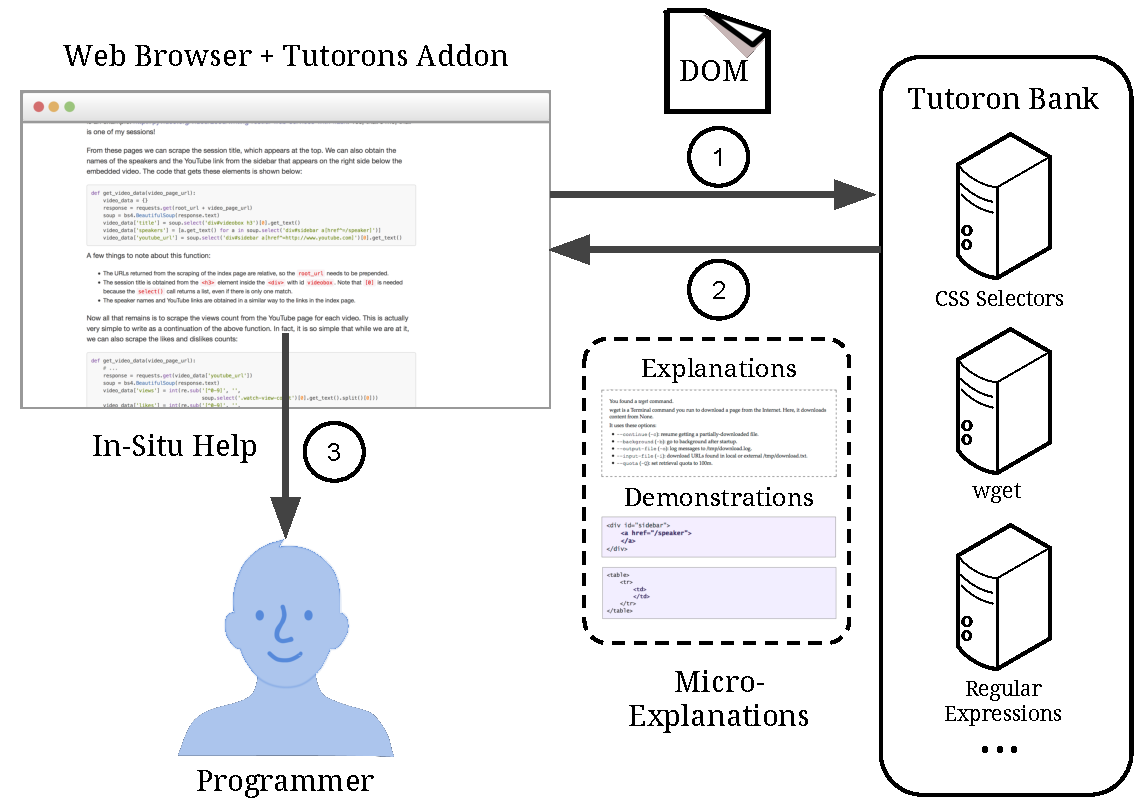
\includegraphics[width=\columnwidth]{figures/tutoron_ecosystem}
    \caption{
    The \Glspl{name} ecosystem and information flow.
    A programmer browses for help in a web browser with the \Glspl{name} addon.
    When she visits a page, the addon queries a bank of \gls{name} servers for different programming languages.
    Each server detects explainable regions of code and produces \glspl{exp}, or explanations and demonstrations of this code.
    The programmer can then view these in-situ and on-demand in tooltip-style overlays by simpling selecting explainable regions of code with the mouse.
    }
    \label{fig:tutoron_ecosystem}
\end{figure}

\if 0
\begin{figure}
\centering
    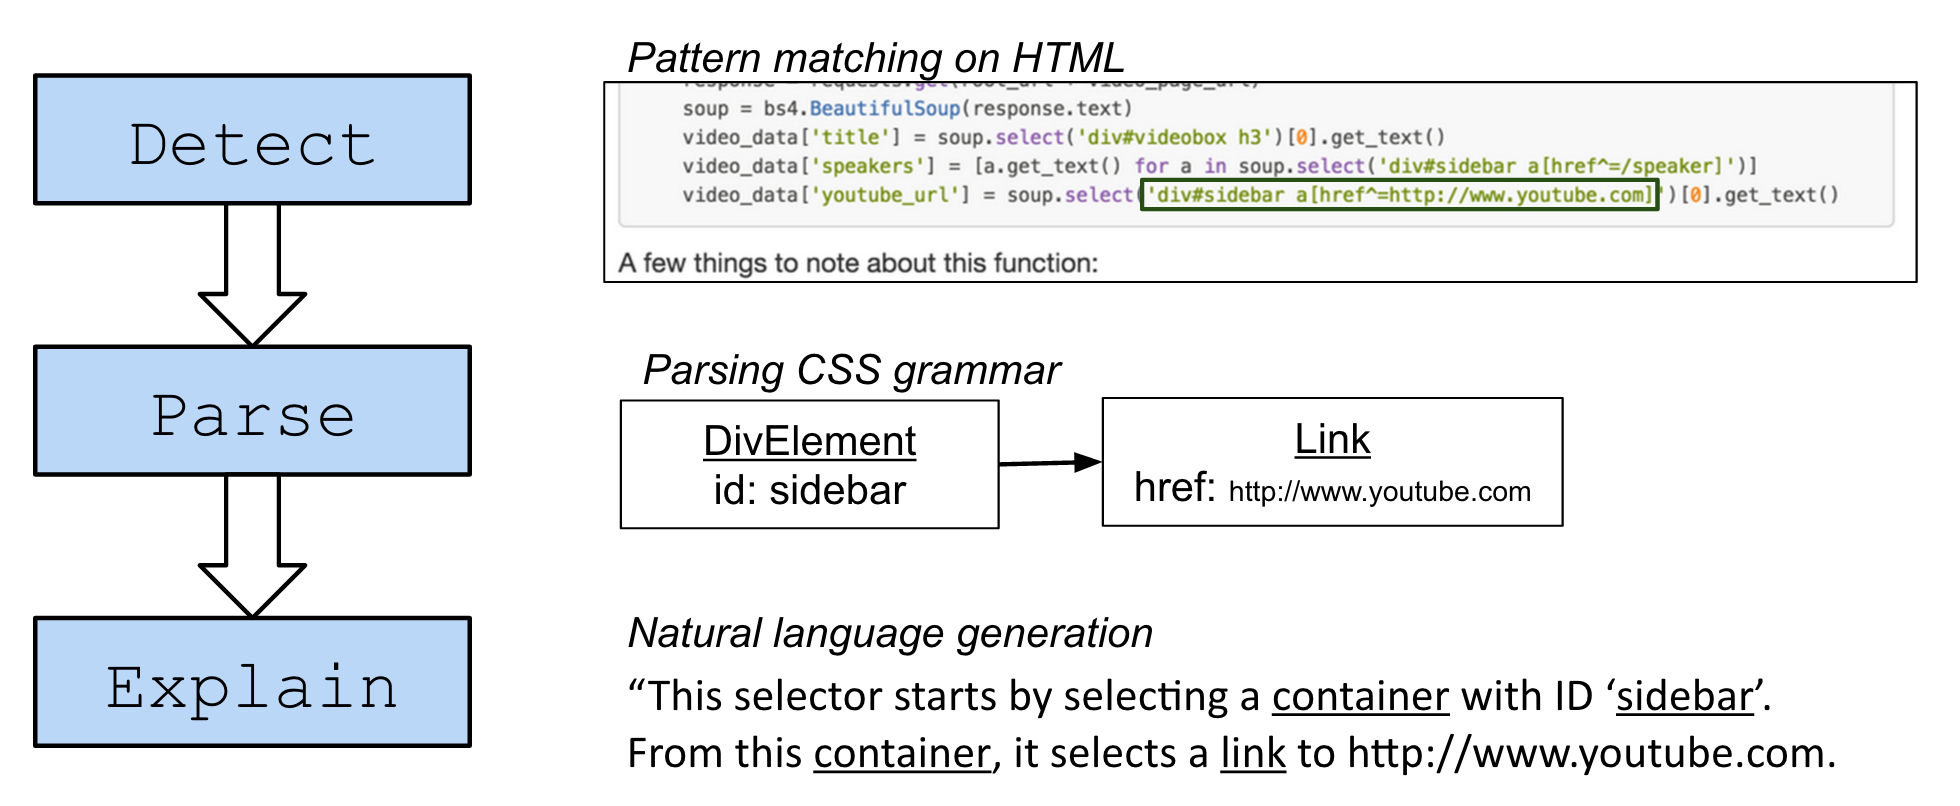
\includegraphics[width=\columnwidth]{figures/explanation_pipeline}
    \caption{\Glspl{name} \emph{detect} relevant code snippets, \emph{parse} them, and then \emph{generate explanations}.  Here we show examples of the output of each stage of the pipeline for a \gls{name} that explains CSS selectors.}
    \label{fig:explanation_pipeline}
\end{figure}
\fi

By installing an addon for the browser, a programmer receives instant access to \glspl{exp}, or in-situ descriptions of code found while browsing, from \gls{name} servers (Figure~\ref{fig:browser_tutorons_markup}).
The addon queries existing \glspl{name} with the page source, receiving micro-explanations for all explainable regions of code.
After receiving explanations, an explanation will appear in a tooltip overlaid on the document directly beneath the source any time the programmer selects an explainable string of text.
The \Glspl{name} addon can query many explanation servers for multi-language support within the same page.
The information flow of the \Glspl{name} ecosystem is shown in Figure~\ref{fig:tutoron_ecosystem}.
We note that our approach could work in other settings, e.g., as a Wordpress plugin, which would shift the burden of installing software from user to tutorial author.

The addon uses a \emph{push} method for fetching explanations rather than a \emph{pull} method, requesting for a server to detect all explainable instances of a language for a webpage.
This choice enables all explanations to be generated in a single batch when the user first accesses the page, reducing the load time to milliseconds instead of seconds to access explanations.
Each server is queried in parallel once the document is ready.
The original webpage is instantly available to the programmer, and \glspl{exp} for each language become available as each \gls{name} processes the DOM.
Computational burden resides on the server, dependent on the implementation.
Client procedures consists of string matching to explainable regions detected followed by insertion of generated HTML into a tooltip, which will be linear in time to the number of explanations.

By requiring \gls{name} servers to detect explainable regions, we resolve the problem where a user's selection may not cover a complete statement of the syntax of a language.
Pre-computing these explainable text regions, we can allow users to select explainable code with \emph{fuzzy boundaries} (see Figure~\ref{fig:fuzzy_boundaries}).
While our qualitative evaluations have shown that this selection mechanism is easy to use, we recognize the future efforts could improve usability.
This includes highlighting explainable regions in colors corresponding to each \gls{name} to indicate what code programmers can gain clarification on, and showing tooltips on hover or right-click events.

\begin{figure}
    \centering
    \framebox{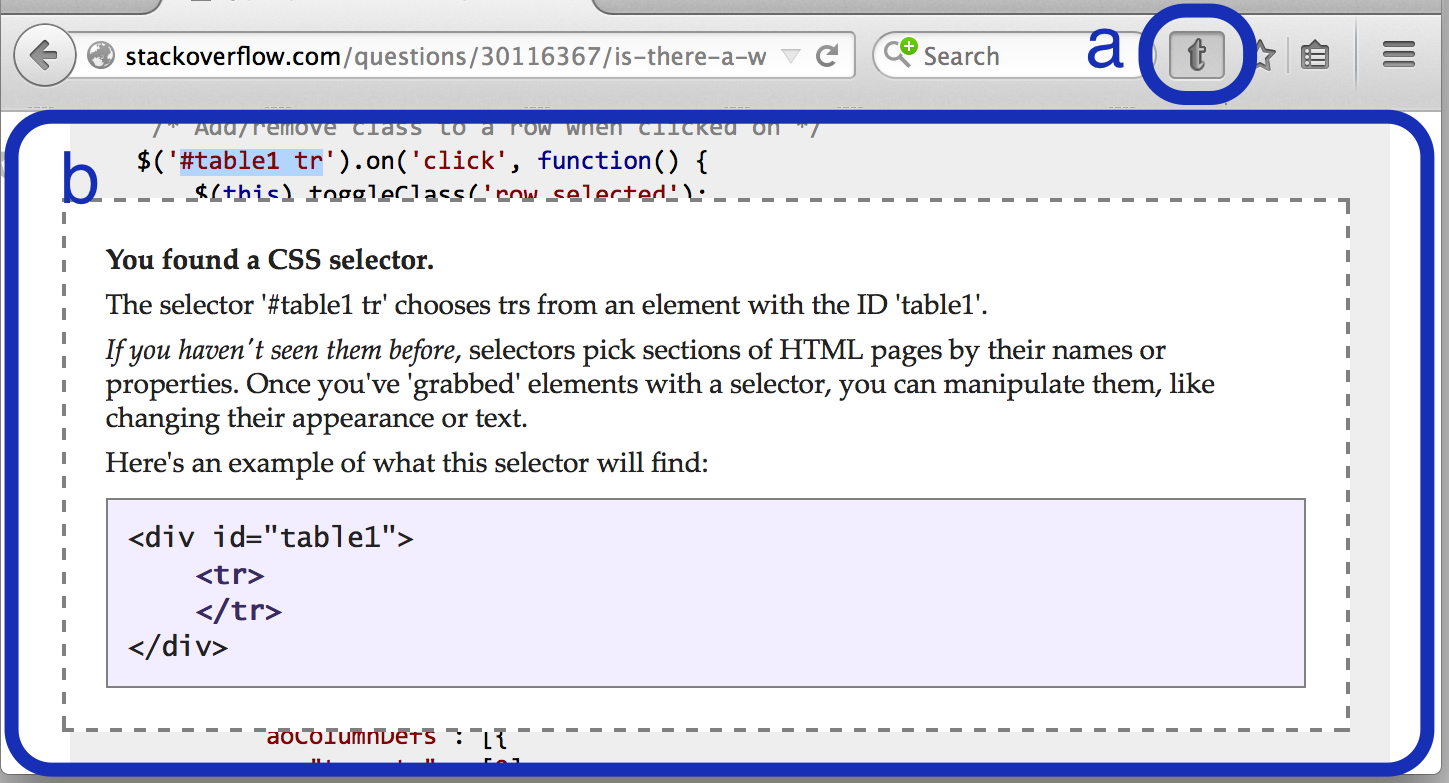
\includegraphics[width=\columnwidth]{figures/browser_tutorons_short}}
    \label{fig:browser_tutorons_markup}
    \caption{A user installs the \Glspl{name} addon.  \emph{(a)} Once she activates it, \emph{(b)} she can view automatically-generated, context-relevant explanations of code of supported languages in-situ while she browses programming help.}
\end{figure}

\begin{figure}
\centering{
    \subfigure[The CSS selector.]{
        \framebox{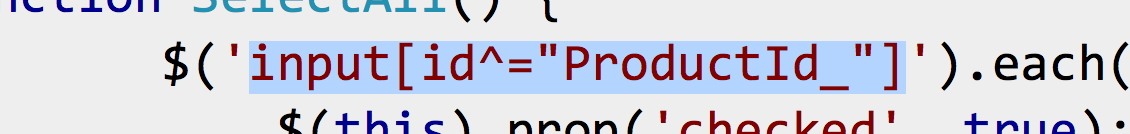
\includegraphics[width=.2\textwidth]{figures/selection_best}}
        \label{fig:selection_best}
    }
    \subfigure[The CSS selector with quotes.]{
        \framebox{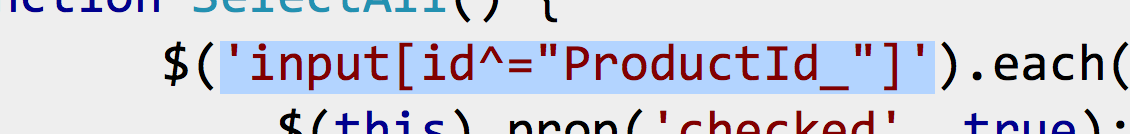
\includegraphics[width=.2\textwidth]{figures/selection_quotes}}
        \label{fig:selection_quotes}
    }
    \subfigure[A jQuery selection.]{
        \framebox{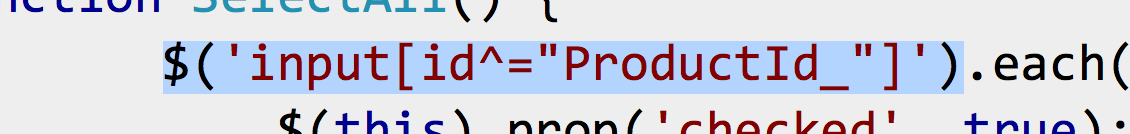
\includegraphics[width=.2\textwidth]{figures/selection_jquery}}
        \label{fig:selection_jquery}
    }
    \subfigure[A sloppy selection.]{
        \framebox{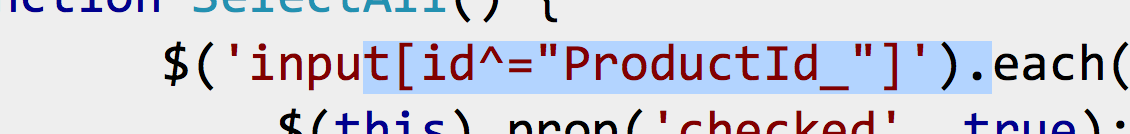
\includegraphics[width=.2\textwidth]{figures/selection_sloppy}}
        \label{fig:selection_sloppy}
    }
    \caption{
    The \Glspl{name} addon activates explanations for code when a user selects text.
    Explainable regions of code are detected on an explanation server and returned to the browser, where the addon enables users to view explanations with fuzzy selections.
    This lets them view \glspl{exp} without knowing the exact syntactic boundaries of the code they want to have described.
    }
    \label{fig:fuzzy_boundaries}
}
\end{figure}

\section{How to Build a \Gls{name}}

A \gls{name} is a routine that \emph{detects}, \emph{parses}, and \emph{explains} code for a specific language in HTML documents.
We describe each processing stage with overarching strategies we have determined for finding relevant code in a page, parsing languages, and generating domain-appropriate explanations.
We couch our discussion in the implementation details of two tutorons we developed for CSS selectors and the \texttt{wget} command and micro-expanations we generate for regular expressions.

\subsection{Detection}
In the \emph{detection} stage, a \gls{name} should extract explainable regions from an HTML document using the language's lexicon and / or syntax.
This can consist of four steps.

First, the \gls{name} extracts blocks of code from HTML pages by selecting code-related elements.
Our current tutorons extract bloks of code from \texttt{<code>} elements, though other common code elements are \texttt{<pre>} and formatted \texttt{<div>} elements.

Second, it divides code blocks into candidate explainable regions based on language-dependent rules.
CSS selectors and regular expressions can be detected as string literals in parsed Python or JavaScript code, requiring an initial parsing stage to detect these candidate regions.
Command lines like \texttt{wget} often occupy a line of a script, meaning that candidate regions can be found by splitting code blocks into lines.

Third, it passes candidate regions through a language-specific syntax checker to determine if it follows the grammar.
Note that if this can be combined with the parsing stage of the \gls{name} processing pipeline.

Finally, a \gls{name} may reduce false positives by filtering candidates to those containing tokens highly representative of the language.
This is necessary when candidate regions are small and the terminals of a grammar accept large character classes.
While the string \texttt{``marti''} in a JavaScript program could represent a custom HTML element we in a selector, it's really more likely a string for some other purpose --- elements in a CSS selector more often than not have tag names defined in the HTML specification (e.g., \texttt{p}, \texttt{div}, or \texttt{img}).

\subsection{Parsing}

Detected code snippets are parsed into a parse tree.
We have found two methods of building parsers to be useful.
When it is necessary to recognize a wide range of symbols and their semantics, \gls{name} authors can modify existing parsers, introducing hooks for extracting results of parsing.
Though this process can be highly involved, requiring a \gls{name} author to have access to the source code and for him to understand how to extract the information and exit the application safely at the appropriate time.
Ultimately, given the involved rules in parsing command lines, this was the right step to take for robust parsing of \texttt{wget} command lines.

However, in other cases, it may be appropriate to develop a custom parser for the language that supports a relevant subset of the language.
For CSS selectors, we wrote a parser in 30 lines of ANTLR\footnote{\url{www.antlr.org}}, which offered several benefits.
First, we had complete control over the parse tree produced.
As our explanations relied on parse tree traversal from leaf element through its parents, we constructed the tree in the format we wanted to traverse.
Second, our parser generator could create tree visitors in both Java and Python, which enabled us to traverse the tree in Java to leverage our natural language software and build example HTML using more familiar Python-based DOM manipulation libraries.
Custom parsers may also be necessary when parser code is too difficult to instrument to extract a useful parse tree, or when source code for the parser is not available.

\subsection{Explanation}

During the final stage, \emph{explanation}, the \gls{name} traverses the parse tree to generate explanations and demonstrations of the code.
The implementation details of this stage is specific to the structure of the parse tree and the ideal representation of the code.
In the next section, we describe techniques that we hope provide inspiration for future language-specific \glspl{exp}.
\section{Evaluation}

\begin{changes}
To evaluate our \glspl{name}, we asked two questions.
First, how reliably can automatic explanations could be generated for the expanse of different formats of online tutorials?
Second, can \glspl{exp} help programmers modify existing, unexplained code without having to consult additional documentation?
We answered the first question through collecting a corpus of online tutorials and measuring the detection accuracy of our \glspl{name} for the languages we support.
We address the second question through an in-lab study with programmers modifying unexplained code to perform new tasks, aided by \glspl{name}.

\subsection{Reliability of Snippet Detection}

To determine the reliabilty of our explainable region detection techniques, we first built a corpus of tutorials that used the languages explained by our \glspl{name}.
For each language, we wanted a diversity of tutorials from different domains.
We attempted to achieve diversity of task addressed in the tutorials for the same language by forming queries from common trigrams of StackOverflow tags containing a language.
For example, fetching the most common tags related to CSS selectors yielded several task-specific trigrams including `css-selectors selenium webdriver' (for client-side application testing) and `css-selectors nokigiri ruby' (for web scraping with Ruby).
For each language, for each of the top trigrams from most popular to least used on StackOverflow, we created a Google query by appending the word `tutorial' to the trigram, fetched the first 10 pages from the search results into our corpus, and stopped after we had fetched 300 tutorials.
After one round of filtering we found that 73\% of CSS selector tutorials, 81\% of wget tutorials, and 76\% of regular expression tutorials had at least some code example and was fetched without a download error, yielding \textgreater 200 tutorials for each language.

We developed a tool to log the locations of manually-selected `ground truth' explainable regions that we found by manually inspecting the tutorials.
Location was stored as a tuple of absolute path to the containing element, and the start and end character indexes of the explainable region within that element.
A match occurred when both the tutoron and a human judge had located an explainable region with exactly the same containing element, and start and end characters.  
`Precision' measured the ratio of correct tutoron detections to the total number of detections, and `recall' measured the ratio of correct tutoron detections to the total number of ground truth explainable regions.

We consistently saw high precision yet low recall with the \glspl{name} (see Table~\ref{tab:detection_accuracy}).    
Low recall can be explained by the fact that code sometimes appears in textual paragraphs, either due to the author's styling preferences, code in unformatted comments at the end of a tutorial, or the author's desire to reference or include a command or abbreviate code snippet in-line with text that describes it.
It is difficult to detect code snippets that are interspersed in textual paragraphs, as there is no textual or structural indicator of where the code starts or ends.
As a result, extra non-code text may be grouped in with the code.
If we restrict \glspl{name} to only scan `code' and `pre' elements on the page, we see an increase in recall to XX-YY\%.
Ultimately, we suspsect that high precision is important to assure \glspl{name} users that the \glspl{exp} illuminate real code, instead of spuriously explaining non-code.
We have yet to verify this experimentally.
While high recall is also important to draw users' attention to explainable code in the browser, \glspl{name} can easily support an architecture where users manually request an explanation for a code snippet that they recognize as being explainable but not automatically detected
\andrew{SIFTER and using machine learning to detect when instances of words are commands.}

\begin{table}
\caption{Accuracy of our explainable region detection.}
\label{tab:detection_accuracy}
\centering
\begin{tabular}{llc}
\toprule
\headrow{Language} & \headrow{Precision} & \headrow{Recall} \\
\midrule
wget & 84\% & 61\% \\ \midrule
CSS selectors & 69\% & 48\% \\ \midrule
RegEx & 78\% & 14\% \\ \bottomrule
\end{tabular}
\end{table}

\subsection{Correctness of Parser}

While our parsers for wget and regular expressions were built on top of existing parsers, we built our simple CSS parser by hand.
We ran our parser against the CSS selectors we extracted from the previous tests as part of our ground truth to see how often it could parse the selectors from the past step without error.
Of the 334 selectors from the last step, 322 (96.4\%) parsed successfully.
Of the 12 that failed to parse, 10 of them could not be lexed as they included incorrectly-formatted characters in the original HTML markup (such as curly quotation marks instead of straight ones) or jQuery-specific pseudo-classes (e.g., \texttt{:jqmData}) that do not belong to the CSS syntax.
With these adjustments, our parser was able to successfully parse 332 our of 334 selectors found online (99.4\%).

\end{changes}

\subsection{In-Lab Usability Study}

We conducted a qualitative usability study to understand how \Glspl{name}-generated \glspl{exp} affected programmers' ability to perform code modification tasks with online example code.
We recruited 9 programmers from university listservs for undergraduate and graduate students in computer science and information science.
All participants had at least two years of programming experience, with a median of 4 years of experience in their longest-used language.  Participants were asked to explain their actions via think-aloud method which was audio-recorded, and their actions were screen-captured and analyzed post-hoc. 

Each participant attempted 8 code modification tasks (plus 2 practice tasks) using two different languages: CSS selectors and \texttt{wget}.
For each language the 4 coding tasks increased in difficulty with the fourth being especially tricky.
We created snippets consisting of a block of code and optionally  explanatory text and comments for each task, based on  existing online programming help.
\begin{changes}
Snippets were from StackOverflow questions or answers.
Tasks asked participants to modify unexplained code from snippets for a purpose unrelated to the StackOverflow question.
\end{changes}
\begin{changes}
While \glspl{name} are designed to help programmers understand code, our tasks focused on code generation and modification.
We see understanding code as central to code modification, and designed tasks to force users to find and understand relevant parts of code.
\end{changes}

Each code modification task consisted of the following steps:
\begin{enumerate}
\item Read a task --- e.g., \emph{write a CSS selector that selects only elements of class \texttt{myInput}.}
\item View a snippet with some clue about the task.
E.g., in Figure~\ref{fig:study_snippet}, the participant was shown a snippet containing CSS selectors that choose elements of class \emph{myCheckbox} without explaining the syntax.
\item Write and test the code in a sandbox we provided.
\end{enumerate}
After reading the snippet, to solve the task, participants could use any resources they wanted to, including searching the web.

\begin{changes}

Example tasks included:
\begin{itemize}

\item
Snippet (excerpt):

\snippet{wget --random-wait -r -p -nd -e robots=off -A``.pdf''  -U mozilla http://math.stanford.edu/undergrad/}

Task: modify the command so it does not automatically fetch the images necessary to display the webpage.

\item
Snippet (excerpt):

\snippet{wget -r -np -N [url] \\}

Task: modify the command to overwrite all files downloaded, even if they have not been updated remotely.

\item

Snippet (excerpt, 1 of 15 lines):

\snippet{\$(`input[id\textasciicircum=``ProductId\_'']')\textbackslash \\  .each(function () \{ }

Task: write a selector that selects only the button elements with IDs starting with bid

\end{itemize}

In one condition, snippets were enhanced with \Glspl{name}.
The \gls{name} did not contain exactly the missing information to complete the task.
For example, for wget tasks, participants were shown descriptions of all options and asked to discover and modify or remove only those relevant to the task.
While these tasks limit the generalizability of our study, we believe that it shows that \Glspl{name} can help in the situations we devised and tested.
\end{changes}

Participants were told they would have 5 minutes for each task; when participants had extra time, if  they had not completed the task, we often asked them to continue so we could observe their problem-solving process. When in the \gls{exp} condition participants were asked to find and view all \glspl{exp} for the source code after reading the snippet.

\begin{figure}
\centering
\framebox{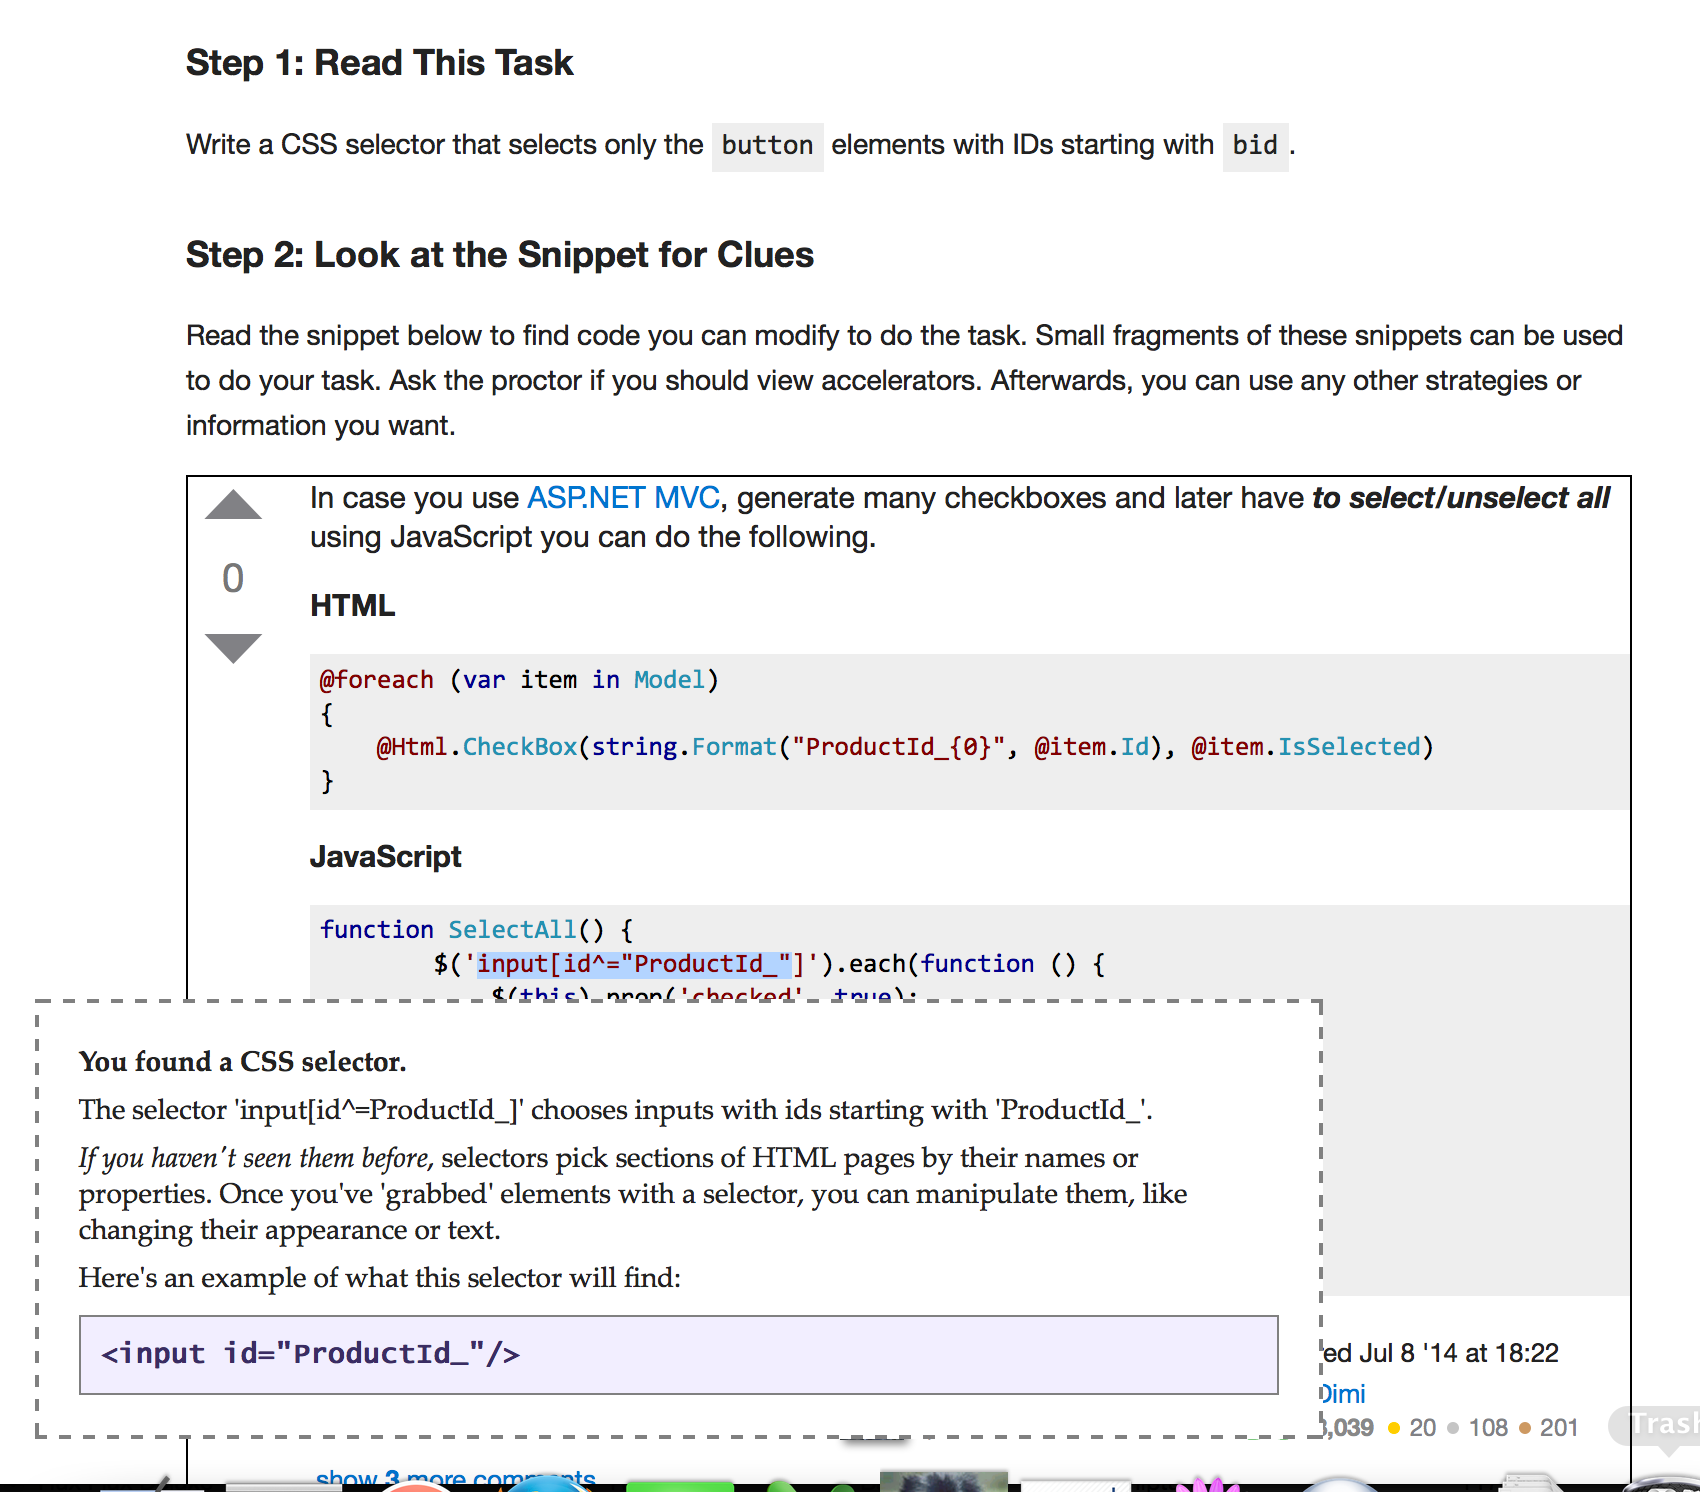
\includegraphics[width=\columnwidth]{figures/study_snippet}}
\caption{An example snippet shown as a clue for a code modification task, accompanied by a \gls{exp} that a participant in our study would have viewed if they were instructed to do so in this task.}
\label{fig:study_snippet}
\end{figure}

Participants viewed \glspl{exp} for alternating tasks so we could observe differences in how they approached the tasks with and without \glspl{exp}; exposure to \glspl{exp} was counter-balanced across participants. 

%%This ordering was counterbalanced across participants so that we could see all tasks performed both with and without \gls{name}-generated \glspl{exp}.

\subsection{Results}

Our primary goal in observing participants was to determine if \gls{name}-generated \glspl{exp} were helpful  during code modification tasks and reduced the need to reference additional documentation.
In the discussion below, we refer to individual participants as $P{1-9}$.

\subsubsection{\Glspl{exp} Help Programmers Modify Code Without Using Other Documentation}

\begin{figure}
\centering
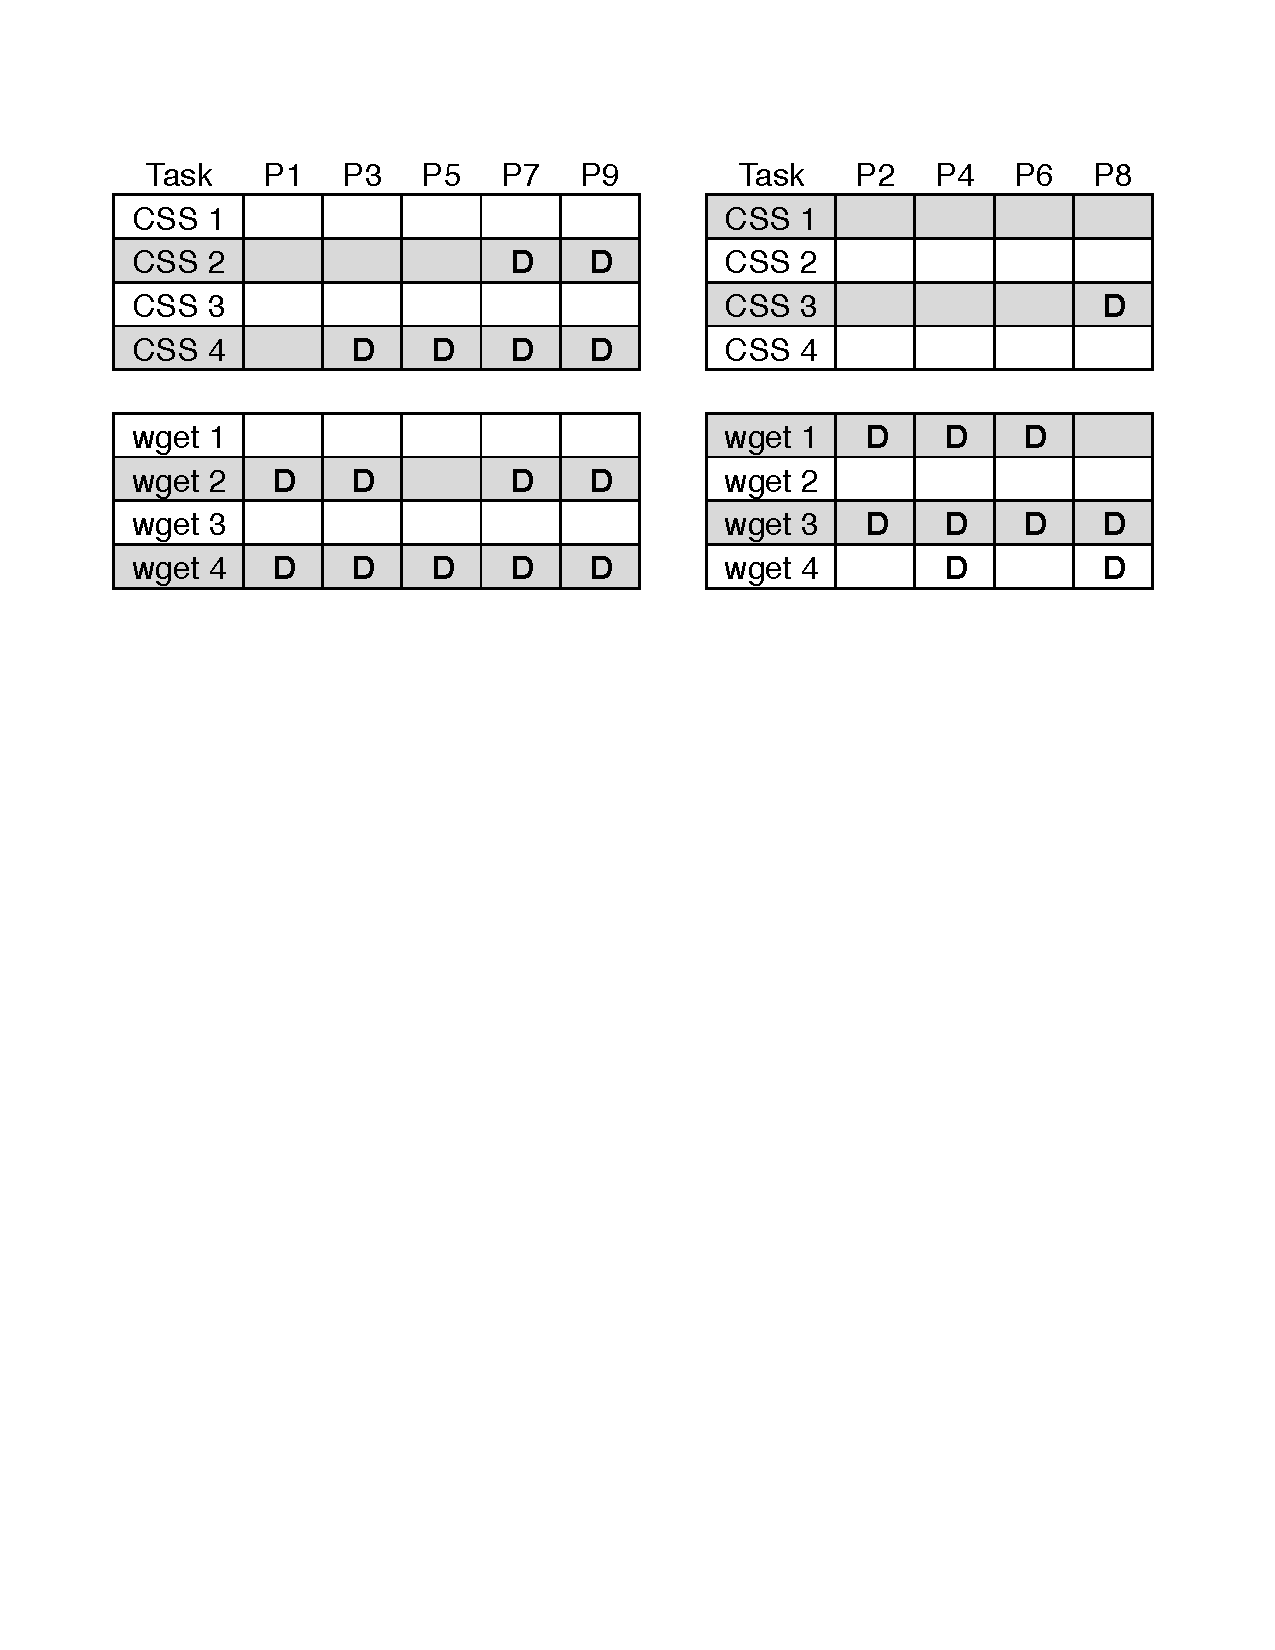
\includegraphics[width=\columnwidth]{figures/doc_accesses}
\caption{%
Tasks for which participants sought additional documentation beyond the snippet. In white rows, participants used \glspl{exp}; in gray rows, they did not.
A cell is marked with the letter `D' if a participant accessed external documentation during that task.
}
\label{fig:doc_accesses}
\end{figure}

When using the \glspl{exp}, 34 out of 36 tasks, or 94\% did not require external documentation.  However, for those tasks where \glspl{exp} were not available, 63\% of the time participants did indeed access external resources in order to complete the task.  The wget tasks especially required external help, with man pages and other resources being accessed in 89\% of cases.  
A detailed breakdown of external document usage is shown in Figure~\ref{fig:doc_accesses}. 


%%In total, out of 72  tasks, participants sought out additional documentation a total of 25 times (Figure~\ref{fig:doc_accesses}).
%%In all wget tasks and in the fourth CSS selector task, a majority of participants without \glspl{name} viewed documentation at some point while trying to find a solution to the problem.
%%In the all 4 CSS selector tasks and the first 3 wget tasks, no participants with access to the \glspl{exp} sought additional documentation in order to solve the problem.

%Only in the final wget task did any participants with access to \glspl{name} seek documentation.


These preliminary results suggest that the \glspl{exp} are effective at reducing the need to switch contexts to find relevant programming help  for completing some programming tasks. 
The \gls{exp} aided the programmers in several ways:

{\bf Reducing need to access external documentation.}
Participants were  able to identify which flags had to be removed from wget commands without consulting external documentation, despite not having used the wget before ($P4$).
For others, the \gls{exp} affirmed a guess that the participant already had about how to construct a CSS selector ($P1$).

{\bf Context-relevant pattern matching.}
One participant noted that the \glspl{exp} helped  to map flags for the wget command line to the higher-level intent of the task ($P4$). 
For the most complex CSS selector task (see Figure~\ref{fig:study_snippet}), two participants noted
that the example HTML shown in the \gls{exp} 
provided a pattern of what fields needed to be changed  from the selector in the snippet to capture the element and ID required by the task prompt ($P2$, $P4$).

{\bf Learning programming concepts.}
For another participant with little previous experience with CSS selectors, a \gls{exp} in  the first task provided him with the knowledge needed to write the selector for the next two tasks, one task for which he was not allowed to view \glspl{exp} ($P5$).

\subsubsection{Programmers Without \Gls{exp} Searched External Documentation}

Some of the difficulties participants faced in the no-\gls{exp} condition  highlight the benefits of in-situ help.
Some participants had difficulty searching for programming help on a web search engine (Google) and using the seach results.
One participant could not express the symbols `\texttt{\^{}=}' as a query term when searching for what  this pattern signifies in CSS selectors.
Her follow-up queries with English language query terms  yielded search results that were not relevant ($P3$).

Participants also had difficulty navigating conventional forms of programming help.
When looking for the \texttt{-r} flag in the man page for wget ($P2$, $P4$), participants found that a page-internal  search for the flag yielded so many matches that it was difficult to find the desired definition.
The description of the \texttt{-N} timestamp flag that was relevant to the code modification task was not directly adjacent to where the flag was introduced, causing one participant to overlook this information, even though it was only 10 lines away ($P3$).

These results underscore the usefulness of context-relevant explanations located within the tutorial text itself.

\subsubsection{Opportunities for Improvement}
In those cases where the \gls{exp} did not aid programmers, there were a few primary causes.

{\bf No visual affordances.} We did not place  visible cues showing where explanations were available.
Programmers may fail to find \glspl{exp} since they have to be explicitly invoked through a right-click.
Although $P2$ eventually found a \gls{exp} that led him to writing a successful CSS selector for the most difficult CSS task, he had to click around the snippet to find it, and did so only upon being reminded by the experimenter that he had not viewed all the \glspl{exp} in the snippet ($P2$).  We plan to experiment with providing visual affordances for the presence of \glspl{exp} in future.


{\bf Selection region ambiguity.}
The leniency of our algorithm for matching a text selection to an explained code fragment caused confusion for programmers about which fragments would be explained on each page ($P1$, $P2$, $P5$).
For the same reason, explanations generated did not always match the fragment selected ($P1$, $P3$, $P5$).
For example, one participant selected the text \texttt{<p>} for which no explanation was generated by the explanation server, because no CSS selector starts with a less-than sign.
However, our selection matching algorithm matched this string to the \texttt{p.mainPageMeters} selector for which an explanation \emph{had} been generated by the server.  As a result, this participant viewed an irrelevant explanation for the code fragment he was viewing ($P5$).  More work is required to determine the right balance of fuzziness for the matching algorithm, with perhaps a drop-down menu of choices for alternative matches.

{\bf Incomplete explanations.} The  \gls{exp} text may not include enough detail to help programmers  develop adequate mental models of unfamiliar material. For instance,
even after completing all 4 CSS selector tasks, $P5$ appeared to believe that CSS selectors were HTML elements themselves, rather than labels that could fetch them, perhaps confused by the example HTML produced in each \gls{exp} ($P5$).  That said, the idea of \gls{exp} can be expanded by adding links to fuller tutorial material.

\section{Discussion}

%%\subsubsection{Evaluating Usability of \Glspl{exp} Interactions}

%%Programmers access \glspl{exp} by selecting code fragments on the page that they want to have explained.
%%In addition, we noted that many of the users selected text when walking through the code during think aloud.
%%Three participants selected code in tasks where \glspl{exp} were disabled when describing either thinking about the code or describing it to the study proctor ($P2$, $P4$, $P5$).
%%One subject even inadvertently brought up an \gls{exp} while pointing out code to the proctor ($P1$).
%%We believe that for some participants, activating the \glspl{exp} by selecting text became a natural, instinctual action.
%%In the final wget task, on subject selected text for a flag he didn't know before remembering that \glspl{exp} were turned off for the task ($P5$).
%%Many participants tried to activate \glspl{exp} to describe single arguments of wget commands ($P2$, $P3$, $P4$, $P5$).
%%This worked in their cases, as there was only ever one code snippet on the page to be explained, and the substring they chose matched the explainable code fragment according to our selection algorithm.

%%However, the leniency of our algorithm for matching a text selection to an explained code fragment caused confusion for programmers about what fragments would be explained on each page ($P1$, $P2$, $P5$).
%%For the same reason, explanations generated did not always match the fragment selected ($P1$, $P3$, $P5$).
%%For example, one user selected the text \texttt{<p>} for which no explanation was generated by the explanation server, as no CSS selector starts with a less-than sign.
%%However, our selection matching algorithm matched this string to the \texttt{p.mainPageMeters} selector for which an explanation \emph{had} been generated by the server.
%%As a result, this user viewed an irrelevant explanation for the code fragment he was viewing ($P5$).

\subsection{Study Caveats}

We are encouraged by the results of this preliminary evaluation of the \gls{exp} idea of context-sensitive programming explanations.
Participants were able to complete the tasks in most cases without requiring other documentation, whereas participants without the explanatory helper text needed to consult external resources.
That said, the study had several limitations.  It consisted of only a small number of participants, and the tasks were designed such that the \Glspl{name} would function properly. 

Furthermore, participants may have been more patient with \gls{exp} content than they would have been with documentation they found on their own, especially if they assumed \glspl{exp} were selected to provide critical insight about the code snippets.
In real world scenarios, programmers may not take the same care in reading the \gls{exp} text as they did in the study.

Finally, tasks in the study involved edit or deletion tasks with existing code.
\Glspl{name} will have to be augmented before they can provide insights for additive tasks and suggest relevant code options that are not in the code itself.

\subsection{Future Work}

\begin{changes}
    When \Glspl{name} are available for many languages, disambiguation between different \Glspl{name} will become necessary as multiple detectors can match a given string.
We see two potential avenues: First, users could explicitly restrict which \Glspl{name} they wish to activate on a given page.
Second, explanations could be ranked by the likeliness that an explainable region belongs to each detected language.
We are currently investigating the use of both rule-based and learned weights based on the frequency of characteristic node types in parse trees as ways of generating these likeliness ratings.
\end{changes}

\if 0
\begin{changes}
In our experience, building reliable detectors requires iterative development and evaluation with a core set of tutorials that use a language.
Collecting a set of test documents, developing the detector, reappropriating parser code, and implmenting an explainer can take dozens of hours.
As the number of languages for which \Glspl{name} would be useful is likely in the dozens, such investments could be appropriate for dedicated members of the larger programmer community, rather than programmers looking for a weekend project.
\end{changes}
\fi

We are also interested in conducting a study with novice programmers.
We believe that observing the problem-solving strategies of novice programmers will yield better recommendations for how to design in-situ help for this group.

\section{Conclusions}

Programmers frequently turn to the web to solve coding problems and to find example code.
\begin{changes}
\Glspl{name} produce explanations for unexplained code that programmers find on the web.
In our framework, \Glspl{name} can produce effective \glspl{exp} when they leverage multiple representations, focus on dynamically generated content, build on existing documentation, and address common usage.
We show that \Glspl{name} for a collection of languages achieve around 80\% accuracy detecting code examples, and improve programmers' ability to modify online code examples without referencing external documentation.
\Glspl{name} bring context-relevant, on-demand documentation to the code examples programmers encounter in online programming documentation.
\end{changes}

\if 0
However, code snippets within  help documentation can contain unexplained concepts that require programmers to seek additional help.
We propose language-specific routines called \Glspl{name} that automatically generate \emph{on-demand, context-relevant} micro-explanations of code.
We demonstrate the technical effort required to build \Glspl{name} by making \gls{exp} for CSS selectors, regular expressions, and Unix commands.
Through a preliminary in-lab study with programmers, we show that these automatically-generated explanations improve participants' ability to modify online code examples without referencing external documentation.
We believe that the \Gls{name} ecosystem will make onine programming examples more understandable and resuable.
\fi


\section*{Acknowledgment}
The authors would like to thank...

% trigger a \newpage just before the given reference
% number - used to balance the columns on the last page
% adjust value as needed - may need to be readjusted if
% the document is modified later
%\IEEEtriggeratref{8}
% The "triggered" command can be changed if desired:
%\IEEEtriggercmd{\enlargethispage{-5in}}

% references section
\bibliographystyle{IEEEtran}
\bibliography{references}

\end{document}
